\section{Heurísticas}

%As que foram implementadas e uma explicação sobre cada uma delas.

O problema de escalonar programas em uma grade de programação de uma emissora de TV a cabo é um caso
particular de um problema bastante conhecido de teoria da combinatória, e que também pode ser visto
como um problema de escalonamento: o \textit{Bin-packing}.

Esse problema é conhecidamente NP-difícil, então não é possível conseguir a solução ótima em um tempo
razoável. Por causa disso, ao invés de tentarmos descobrir a solução ótima, temos que ir atrás de uma
solução que é apenas satisfatória, uma aproximação. Para conseguir uma aproximação precisamos usar
heurísticas.

Heurísticas são algoritmos de aproximação, ou seja, algoritmos que não buscam encontrar a solução ótima,
mas uma solução que consiga se aproximar da ótima segundo algum fator. Esse fator é a razão entre
a solução aproximada e a ótima, significando o quão boa é a aproximação.

Uma característica importante de heurísticas é que elas tomam decisões específicas quando chegam em determinado
ponto do algoritmo. Por exemplo escolher o maior item, inverter a ordem de itens da solução, etc.

Para conseguir uma solução aproximada para o problema \textit{Bin-packing} podemos utilizar várias heurísticas.
Algumas delas foram implementadas e rodadas com a mesma entrada.

\subsection{First Fit}

O \textit{First Fit} coloca o item no primeiro bin em que ele cabe. No caso do problema da grade de programação,
o programa é colocando no primeiro dia em que ele cabe. Caso o programa não caiba em nenhum dos dias, é criado
um novo dia.

\begin{figure}[H]
  \centering
  \fbox{
    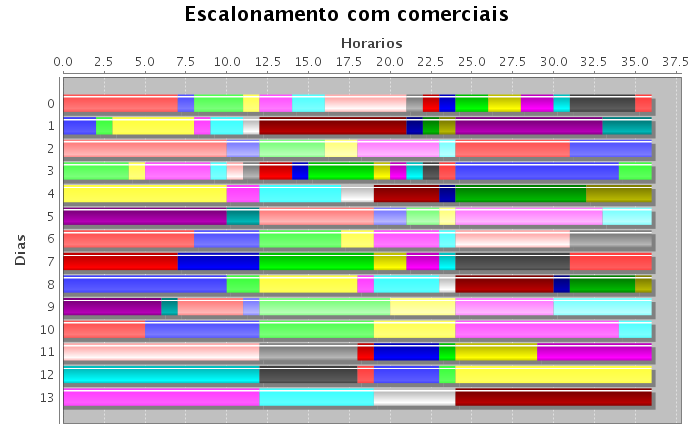
\includegraphics[width=110mm]{first-fit.png}
  }
  \caption{Resolução de um problema usando o First Fit}
\end{figure}

\subsection{First Fit Decreasing}

O \textit{First Fit Decreasing} é uma variação do First Fit em que os itens são ordenados em ordem decrescente
de valor antes de rodar o algoritmo. Essa heurística só pode ser usada se todos os itens forem conhecidos de
antemão.

\begin{figure}[H]
  \centering
  \fbox{
    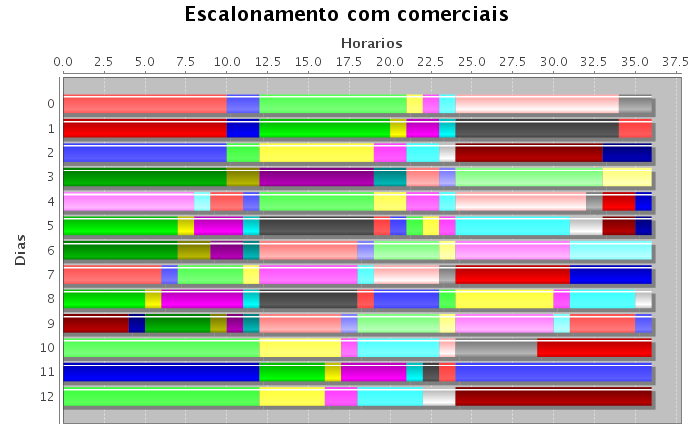
\includegraphics[width=110mm]{first-fit-dec.png}
  }
  \caption{Resolução de um problema usando o First Fit Decreasing}
\end{figure}

\subsection{Next Fit}

O \textit{Next Fit} tenta preencher um bin usando o primeiro item que caiba, se nenhum programa couber, um
novo bin é criado. A principal diferença entre o \textit{Next Fit} e o \textit{First Fit} é que no primeiro
é preenchido um bin por vez e no segundo tenta-se colocar o item no primeiro bin que ele caiba.

\begin{figure}[H]
  \centering
  \fbox{
    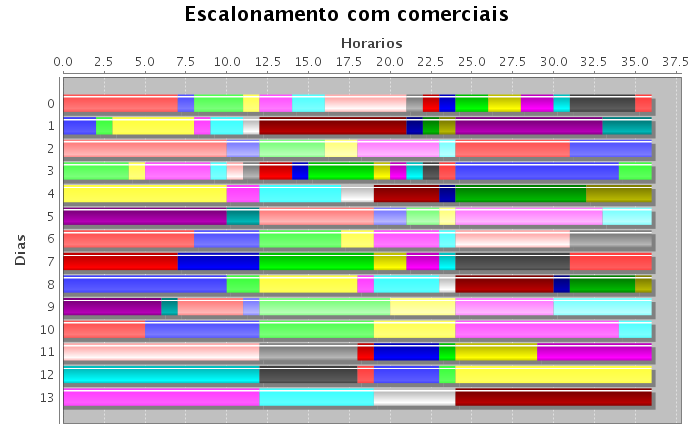
\includegraphics[width=110mm]{first-fit.png}
  }
  \caption{Resolução de um problema usando o Next Fit}
\end{figure}

\subsection{Best Fit}

O \textit{Best Fit} tenta colocar o item no bin em que, após colocar o item, sobre o mínimo de espaço restante
no bin. Caso não caiba em nenhum bin, é criado um novo.

\begin{figure}[H]
  \centering
  \fbox{
    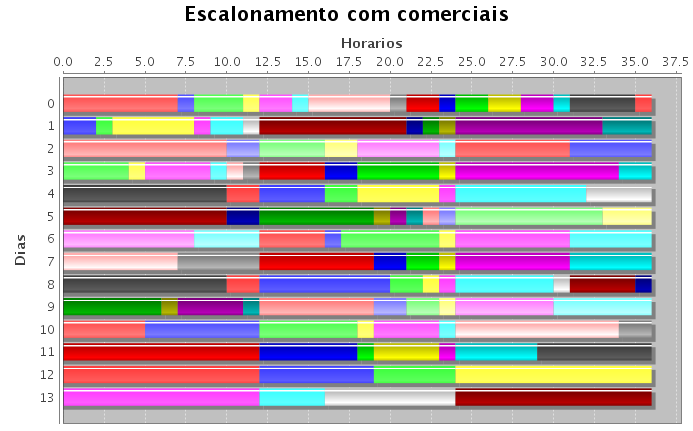
\includegraphics[width=110mm]{best-fit.png}
  }
  \caption{Resolução de um problema usando o Best Fit}
\end{figure}

\subsection{Best Fit Decreasing}

O \textit{Best Fit Decreasing} é uma variação do \textit{Best Fit} em que os itens são ordenados em ordem
decrescente de valor antes de rodar o Algoritmo.

\begin{figure}[H]
  \centering
  \fbox{
    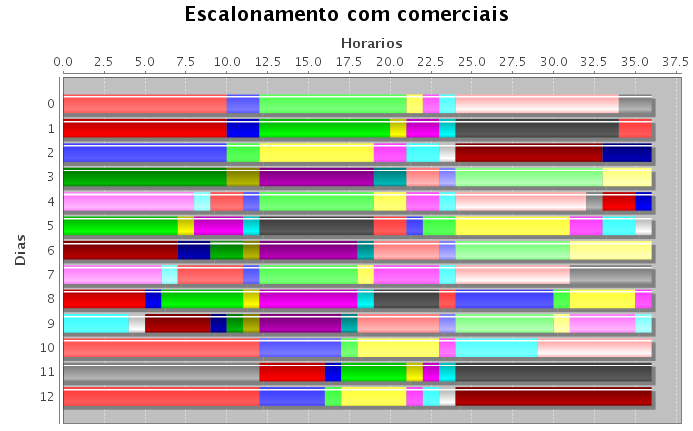
\includegraphics[width=110mm]{best-fit-dec.png}
  }
  \caption{Resolução de um problema usando o Best Fit Decreasing}
\end{figure}

\subsection{Worst Fit}

O \textit{Worst Fit} tenta colocar o item no bin em que, após colocar o item, sobre o máximo de espaço restante
no bin. Caso não caiba em nenhum bin, é criado um novo.

\begin{figure}[H]
  \centering
  \fbox{
    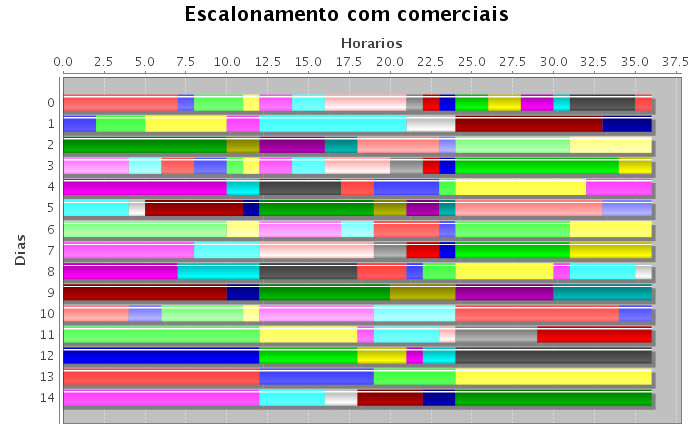
\includegraphics[width=110mm]{worst-fit.png}
  }
  \caption{Resolução de um problema usando o Worst Fit}
\end{figure}

\subsection{Almost Worst Fit}

O \textit{Almost Worst Fit} é semelhante ao \textit{Worst Fit}, mas escolhe-se o bin que tem o segundo maior
espaço restante. Caso caiba em apenas um bin o item é colocado nele, e caso não caiba em nenhum, um novo bin
é criado.

\begin{figure}[H]
  \centering
  \fbox{
    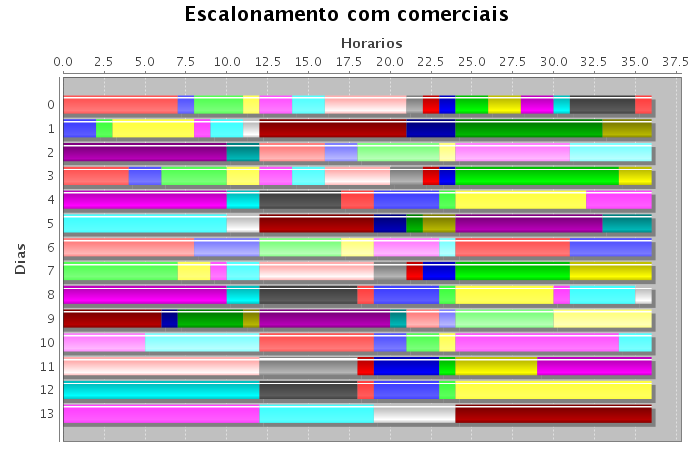
\includegraphics[width=110mm]{almost-worst-fit.png}
  }
  \caption{Resolução de um problema usando o Almost Worst Fit}
\end{figure}

